% !Mode:: "TeX:UTF-8"
% !TEX program  = pdflatex
\documentclass[a4paper]{article}

% import settings, modify the number of homework in this file

\usepackage[T1]{fontenc}
\usepackage{amsmath, amssymb, amsthm}
% amsmath: equation*, amssymb: mathbb, amsthm: proof
\usepackage{moreenum}
\usepackage{mathtools}
\usepackage{url}
\usepackage{graphicx}
\usepackage{subcaption}
\usepackage{booktabs} 
\usepackage[mathcal]{eucal}
\usepackage{dsfont}
\usepackage{geometry}
\geometry{left=30mm,right=30mm,	top=42mm, bottom=33mm}

\usepackage[numbered,framed]{matlab-prettifier}
\lstset{
	style              = Matlab-editor,
	captionpos         =b,
	basicstyle         = \mlttfamily,
	escapechar         = ",
	mlshowsectionrules = true,
}

% set the homework count number
\usepackage[thehwcnt = 1]{iidef}

\newcommand\dif{\text{d}}
\newcommand\no{\noindent}
\newcommand\dis{\displaystyle}
\newcommand\ls{\leqslant}
\newcommand\gs{\geqslant}

\newcommand\limit{\dis\lim\limits}
\newcommand\limn{\dis\lim\limits_{n\to\infty}}
\newcommand\limxz{\dis\lim\limits_{x\to0}}
\newcommand\limxi{\dis\lim\limits_{x\to\infty}}
\newcommand\limxpi{\dis\lim\limits_{x\to+\infty}}
\newcommand\limxni{\dis\lim\limits_{x\to-\infty}}
\newcommand\limtpi{\dis\lim\limits_{t\to+\infty}}
\newcommand\limtni{\dis\lim\limits_{t\to-\infty}}

\newcommand\sumn{\dis\sum\limits_{n=1}^{\infty}}
\newcommand\sumnz{\dis\sum\limits_{n=0}^{\infty}}

\newcommand\sumi{\dis\sum\limits_{i=1}^{\infty}}
\newcommand\sumiz{\dis\sum\limits_{i=0}^{\infty}}
\newcommand\sumin{\dis\sum\limits_{i=1}^{n}}
\newcommand\sumizn{\dis\sum\limits_{i=0}^{n}}

\newcommand\sumk{\dis\sum\limits_{k=1}^{\infty}}
\newcommand\sumkz{\dis\sum\limits_{k=0}^{\infty}}
\newcommand\sumkn{\dis\sum\limits_{k=0}^n}
\newcommand\sumkfn{\dis\sum\limits_{k=1}^n}

\newcommand\pzx{\dis\frac{\partial z}{\partial x}}
\newcommand\pzy{\dis\frac{\partial z}{\partial y}}

\newcommand\pfx{\dis\frac{\partial f}{\partial x}}
\newcommand\pfy{\dis\frac{\partial f}{\partial y}}

\newcommand\pzxx{\dis\frac{\partial^2 z}{\partial x^2}}
\newcommand\pzxy{\dis\frac{\partial^2 z}{\partial x\partial y}}
\newcommand\pzyx{\dis\frac{\partial^2 z}{\partial y\partial x}}
\newcommand\pzyy{\dis\frac{\partial^2 z}{\partial y^2}}

\newcommand\pfxx{\dis\frac{\partial^2 f}{\partial x^2}}
\newcommand\pfxy{\dis\frac{\partial^2 f}{\partial x\partial y}}
\newcommand\pfyx{\dis\frac{\partial^2 f}{\partial y\partial x}}
\newcommand\pfyy{\dis\frac{\partial^2 f}{\partial y^2}}

\newcommand\intzi{\dis\int_{0}^{+\infty}}
\newcommand\intd{\dis\int}
\newcommand\intab{\dis\int_a^b}

\newcommand{\degree}{^\circ}

\newcommand\ma{\mathcal{A}}
\newcommand\mb{\mathcal{B}}
\newcommand\mc{\mathcal{C}}
\newcommand\me{\mathcal{E}}
\newcommand\mg{\mathcal{g}}

\newcommand\mcc{\mathbb{C}}
\newcommand\mrr{\mathbb{R}}
\newcommand\mzz{\mathbb{Z}}

\newcommand\mx{\bf{x}}
\newcommand\mX{\bf{X}}
\newcommand\my{\bf{y}}
\newcommand\mY{\bf{Y}}
%%=============================================

%%=====定义新数学符号===============================
\DeclareMathOperator{\sgn}{sgn}
\DeclareMathOperator{\arccot}{arccot}
\DeclareMathOperator{\arccosh}{arccosh}
\DeclareMathOperator{\arcsinh}{arcsinh}
\DeclareMathOperator{\arctanh}{arctanh}
\DeclareMathOperator{\arccoth}{arccoth}
\DeclareMathOperator{\grad}{\bf{grad}}
%\DeclareMathOperator{\argmax}{argmax}
%\DeclareMathOperator{\argmin}{argmin}
%\DeclareMathOperator{\diag}{diag}
\DeclareMathOperator{\csign}{csign}
%===============================================

\thecourseinstitute{Harbin Institute of Technology, ShenZhen}
\thecoursename{Operations Research}
\theterm{Fall 2019}
\hwname{Homework}

\begin{document}
\courseheader
\name{JingXuan Yang, SZ160310217}

\begin{enumerate}
  \setlength{\itemsep}{3\parskip}

% first exercise
  \item The Versatech Corporation has decided to produce three new products. Five branch plants now have excess product capacity. The unit manufacturing cost of the first product would be \$31, \$29, \$32, \$28, and \$29 in Plants 1, 2, 3, 4, and 5, respectively. The unit manufacturing cost of the second product would be \$45, \$41, \$46, \$42, and \$43 in Plants 1, 2, 3, 4, and 5, respectively. The unit manufacturing cost of the third product would be \$38, \$35, and \$40 in Plants 1, 2, and 3, respectively, whereas Plants 4 and 5 do not have the capability for producing this product. Sales forecasts indicate that 600, 1000, and 800 units of products 1, 2, and 3, respectively, should be produced per day. Plants 1, 2, 3, 4, and 5 have the capacity to produce 400, 600, 400, 600, and 1000 units daily, respectively, regardless of the product or combination of products involved. Assume that any plant having the capability and capacity to produce them can produce any combination of the products in any quantity.
  
  \hspace*{4ex}Management wishes to know how to allocate the new products to the plants to minimize total manufacturing cost.
  
  \hspace*{4ex}Formulate this problem as a transportation problem by constructing the appropriate parameter table.
  \begin{solution}
  	First identify parameter variables:
   \begin{equation*}
   \begin{aligned}
   \text{Source }i&=\text{Production of products in plant }i,\ i=1,2,3,4,5\\
   \text{Destination }j&=\text{Sales of product }j,\ j=1,2,3\\
   x_{ij}&=\text{number of products produced in plant } i \text{ for sales of product } j\\
   c_{ij}&=\text{cost associated with each unit of }x_{ij}\\
   s_i&=\text{number of products produced in plant }i\\
   d_j&=\text{number of products for sales of product } j\\
   \end{aligned}
   \end{equation*}
   Since the total supply is larger than total demand by 600, we introduce a dummy destination (Dummy 4) to receive the surplus products.
   
   \hspace*{4ex}The parameter table is shown in Tab.\ref{tab1}.
   \begin{table}[h]
   	\centering
   	\caption{Parameter table for Versatech Corporation}
   	\label{tab1}
   	\begin{tabular}{llccccc}
   		\toprule[1.5pt]
   		&&\multicolumn{4}{c}{Destination}&\\
   		\cmidrule{3-6}
   		&&Product 1&Product 2&Product 3&Dummy 4&Supply\\
   		\midrule
   		\multirow{5}{*}{Source}&Plant 1& 31& 45& 38&0&400\\
   		&Plant 2& 29& 41& 35&0&600\\
   		&Plant 3& 32& 46& 40&0&400\\
   		&Plant 4& 28& 42&$M$&0&600\\
   		&Plant 5& 29& 43&$M$&0&1000\\
   		\multicolumn{2}{l}{Demand} &600&1000&800&600&\\   	
   		\bottomrule[1.5pt]
   	\end{tabular}
   \end{table}
  \end{solution}

\newpage

\item The Energetic Company needs to make plans for the energy systems for a new building. The energy needs in the building fall into three categories: (1) electricity, (2) heating water, and (3) heating space in the building. The daily requirements for these three categories (all measured in the same units) are
\begin{table}[h]
	\centering
	\begin{tabular}{lr}
		\toprule[1.5pt]
		Electricity&20 units\\
		Water heating&10 units\\
		Space heating&30 units\\
		\bottomrule[1.5pt]
	\end{tabular}
\end{table}

The three possible sources of energy to meet these needs are electricity, natural gas, and a solar heating unit that can be installed on the roof. The size of the roof limits the largest possible solar heater to 30 units, but there is no limit to the electricity and natural gas available. Electricity needs can be met only by purchasing electricity (at a cost of \$50 per unit). Both other energy needs can be met by any source or combination of sources. The unit costs are
\begin{table}[h]
	\centering
	\begin{tabular}{cccc}
		\toprule[1.5pt]
		&Electricity&Natural Gas&Solar Heater\\
		\midrule
		Water heating&\$90&\$60&\$30\\
		Space heating&\$80 &\$50 &\$40\\
		\bottomrule[1.5pt]
	\end{tabular}
\end{table}

The objective is to minimize the total cost of meeting the energy needs.
\begin{enumerate}
	\item Formulate this problem as a transportation problem by constructing the appropriate parameter table. (Hint: Since there is no limit to the electricity and natural gas available, let the supply of electricity be the sum of demands for electricity, water and space heating, and let the supply of natural gas be the sum of demands for water and space heating.)
	\begin{solution}
		
		First identify parameter variables:
		\begin{equation*}
		\begin{aligned}
		\text{Source }i&=\text{Energy supplies }i,\ i=1,2,3\\
		\text{Destination }j&=\text{Energy needs }j,\ j=1,2,3\\
		x_{ij}&=\text{number of energy need } i \text{ provided by energy supply } j\\
		c_{ij}&=\text{cost associated with each unit of }x_{ij}\\
		s_i&=\text{number of energy units produced by energy supply }i\\
		d_j&=\text{number of energy units for energy need } j\\
		\end{aligned}
		\end{equation*}
		Since the total supply is larger than total demand by 70, we introduce a dummy destination to receive the surplus energy units.
		
		\hspace*{4ex}The parameter table is shown in Tab.\ref{tab2}.
		\begin{table}[H]
			\centering
			\caption{Parameter table for Energetic Company}
			\label{tab2}
			\begin{tabular}{llccccc}
				\toprule[1.5pt]
				&&\multicolumn{4}{c}{Destination}&\\
				\cmidrule{3-6}
				&&Electricity&Water heating&Space heating&Dummy&Supply\\
				\midrule
				\multirow{3}{*}{Source}
				&Electricity& 50& 90& 80&0&60\\
				&Natural gas& $M$&60& 50&0&40\\
				&Solar heater& $M$&30& 40&0&30\\
				\multicolumn{2}{l}{Demand} &20&10&30&70&\\   	
				\bottomrule[1.5pt]
			\end{tabular}
		\end{table}
		
	\end{solution}
	\vspace*{-1cm}
	\item Use the northwest corner rule to obtain an initial BF solution for this problem, and identify whether the initial BF solution is optimal. If the initial BF solution is not optimal, start with it and complete the first iteration of the transportation simplex method.
	\begin{solution}
		The initial BF solution obtained by northwest method is shown in Tab.\ref{tab3}.
		\begin{table}[h]
			\caption{Initial BF solution by northwest method}
			\label{tab3}
			\centering
			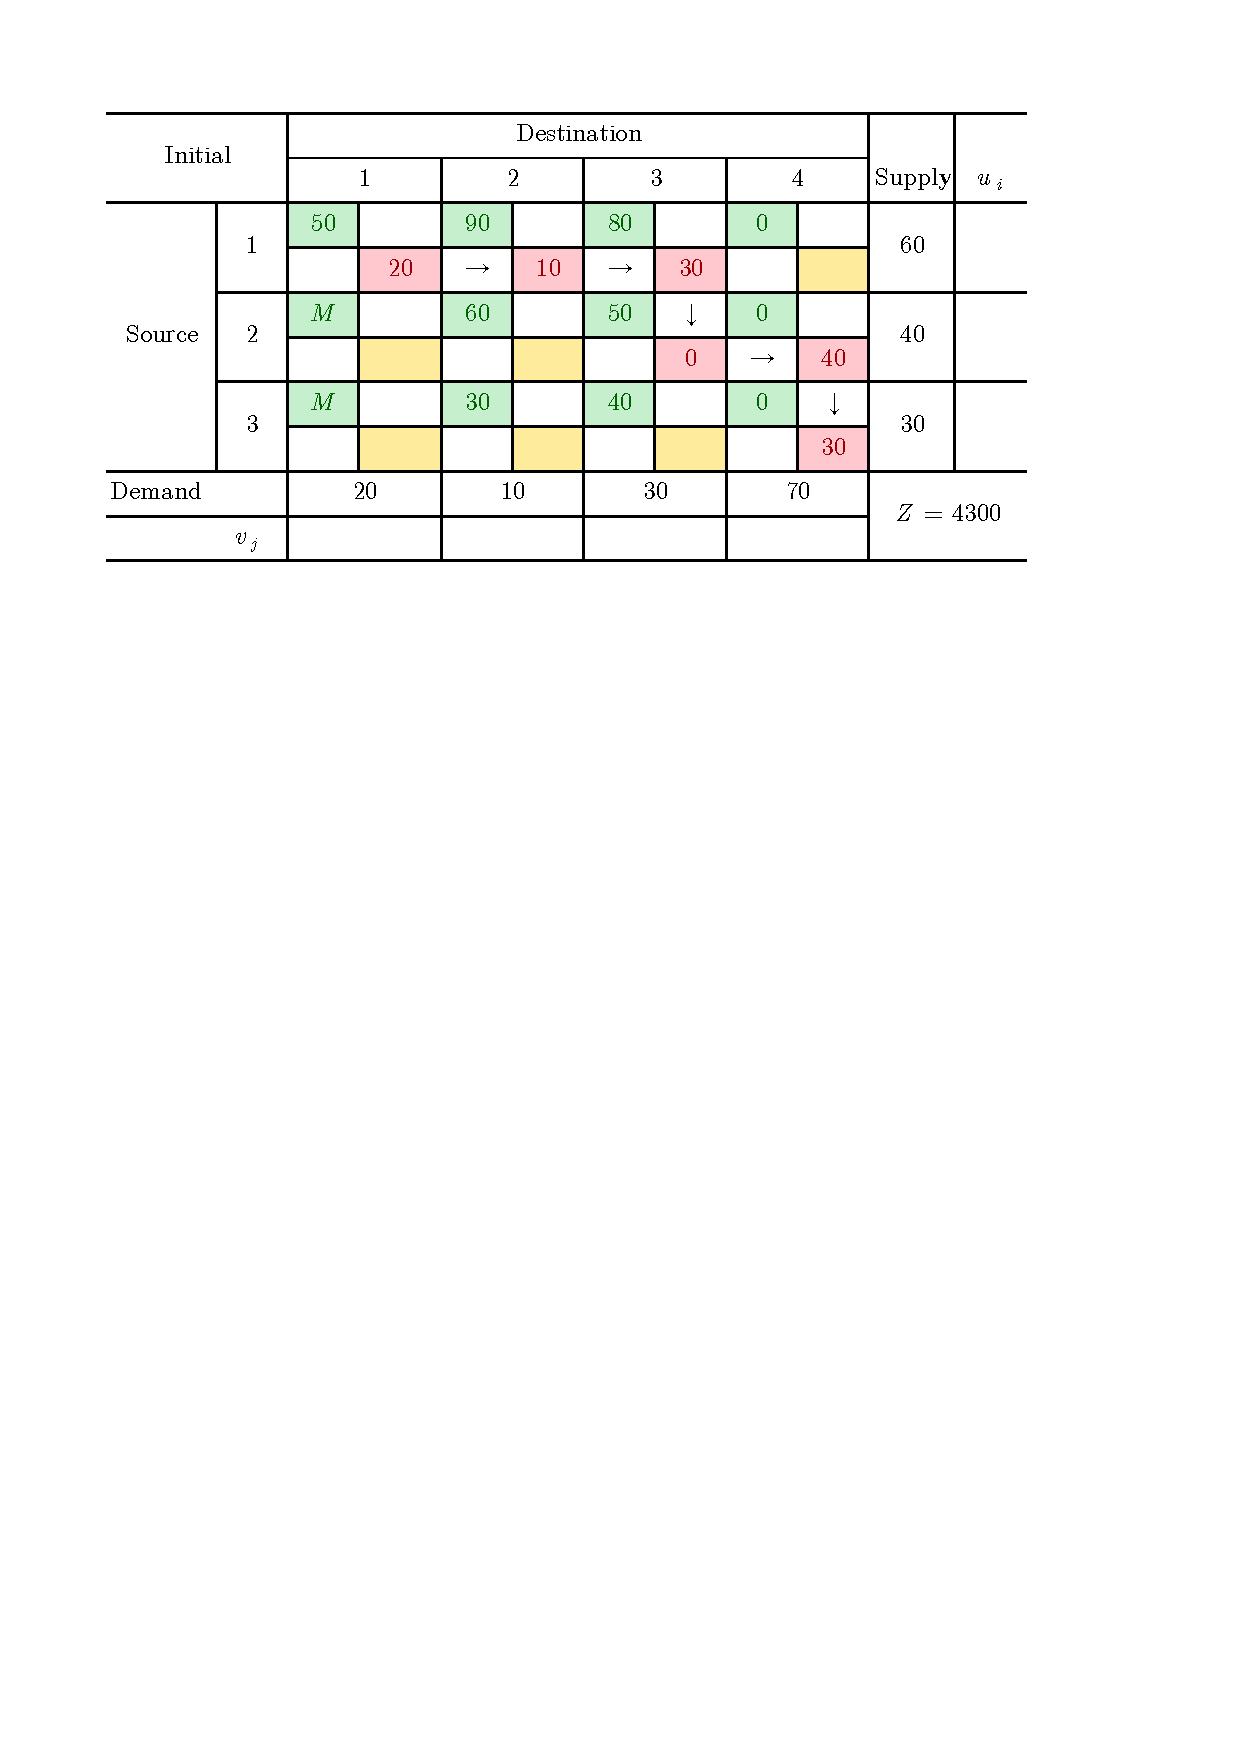
\includegraphics[width = 0.8\textwidth]{NW1}				
		\end{table}
		
		\textit{Optimality test}
		
		The completed initial transportation simplex tableau is shown in Tab.\ref{tab4}.
		\begin{table}[h]
			\caption{Completed initial transportation simplex tableau}
			\label{tab4}
			\centering
			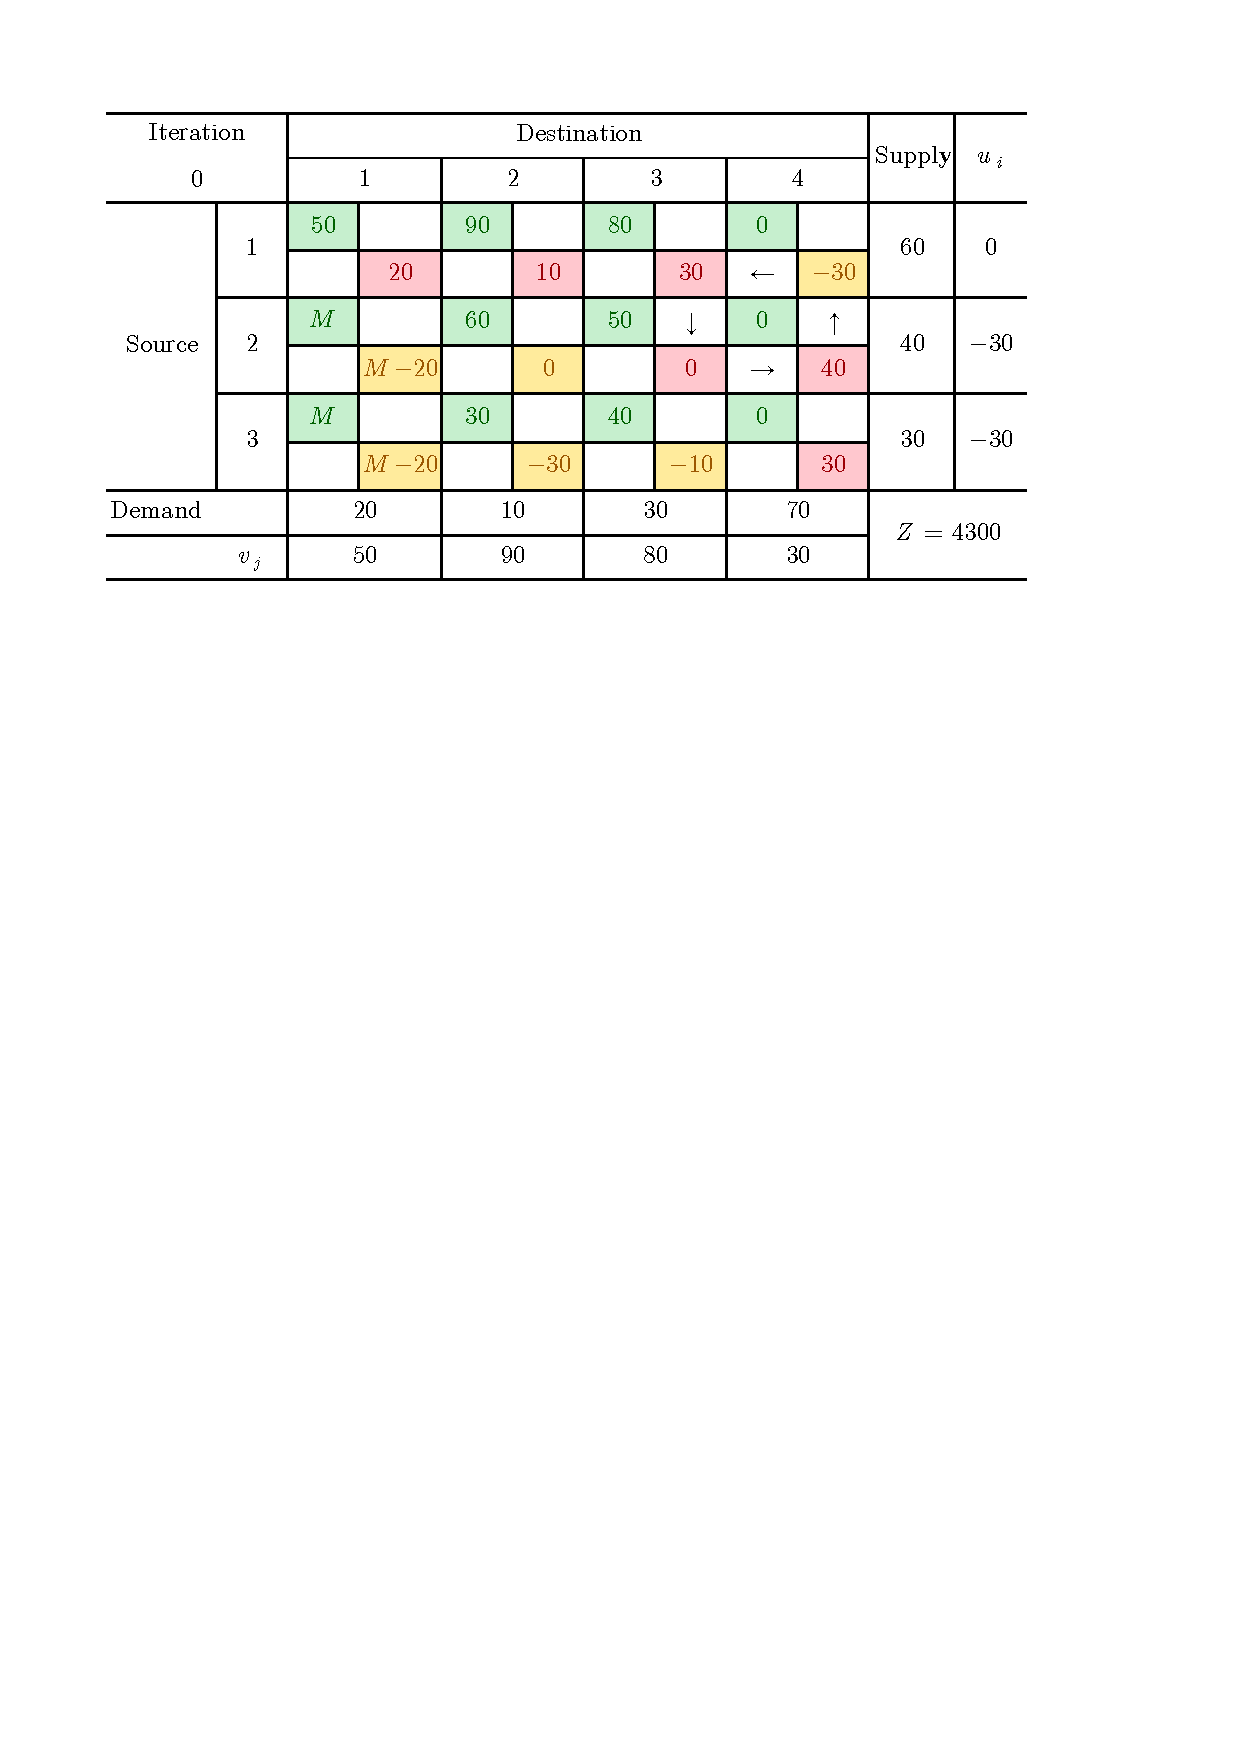
\includegraphics[width = 0.8\textwidth]{NW2}				
		\end{table}
	
	    There are negative nonbasic variables, thus it's not optimal. There exists two elements that equal $-30$, we choose $x_{14}$ as the entering basic variable, since the chain of $x_{14}$ is simpler. Because $x_{13}=30$ first decreases to zero, we choose $x_{13}$ to be the leaving basic variable.
		
		\hspace*{4ex}The change in objective function is
		\begin{equation*}
		\Delta Z=30\times(0-80+50-0)=-900
		\end{equation*}
		This first iteration is shown in Tab.\ref{tab5}.
		
		\begin{table}[H]
			\caption{First iteration of transportation simplex tableau}
			\label{tab5}
			\centering
			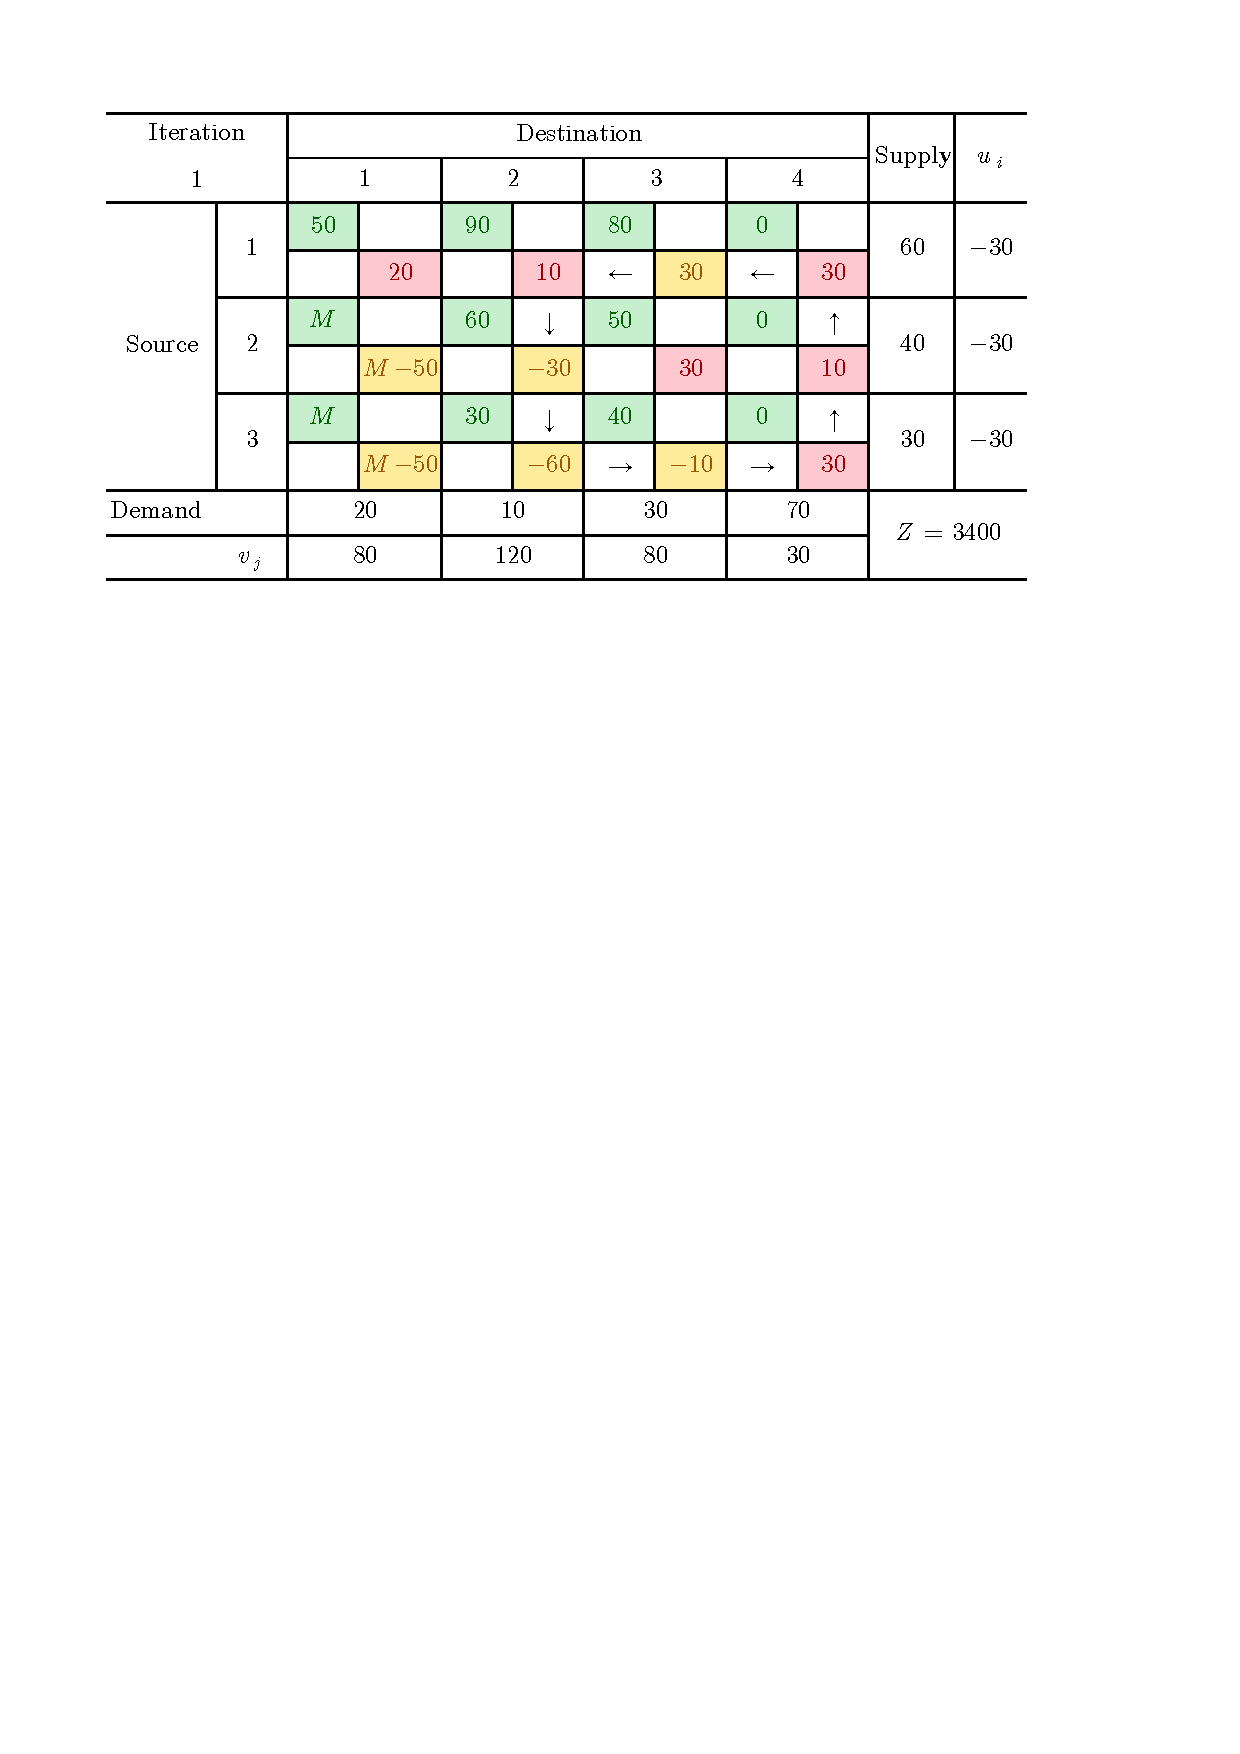
\includegraphics[width = 0.75\textwidth]{NW3}				
		\end{table}

		
		Although the homework does not require to find the optimal solution, we go on above procedures to find it, shown in Tab.\ref{tabNW4} and Tab.\ref{tabNW5}.
		
			\begin{table}[H]
			\caption{Second iteration of transportation simplex tableau}
			\label{tabNW4}
			\centering
			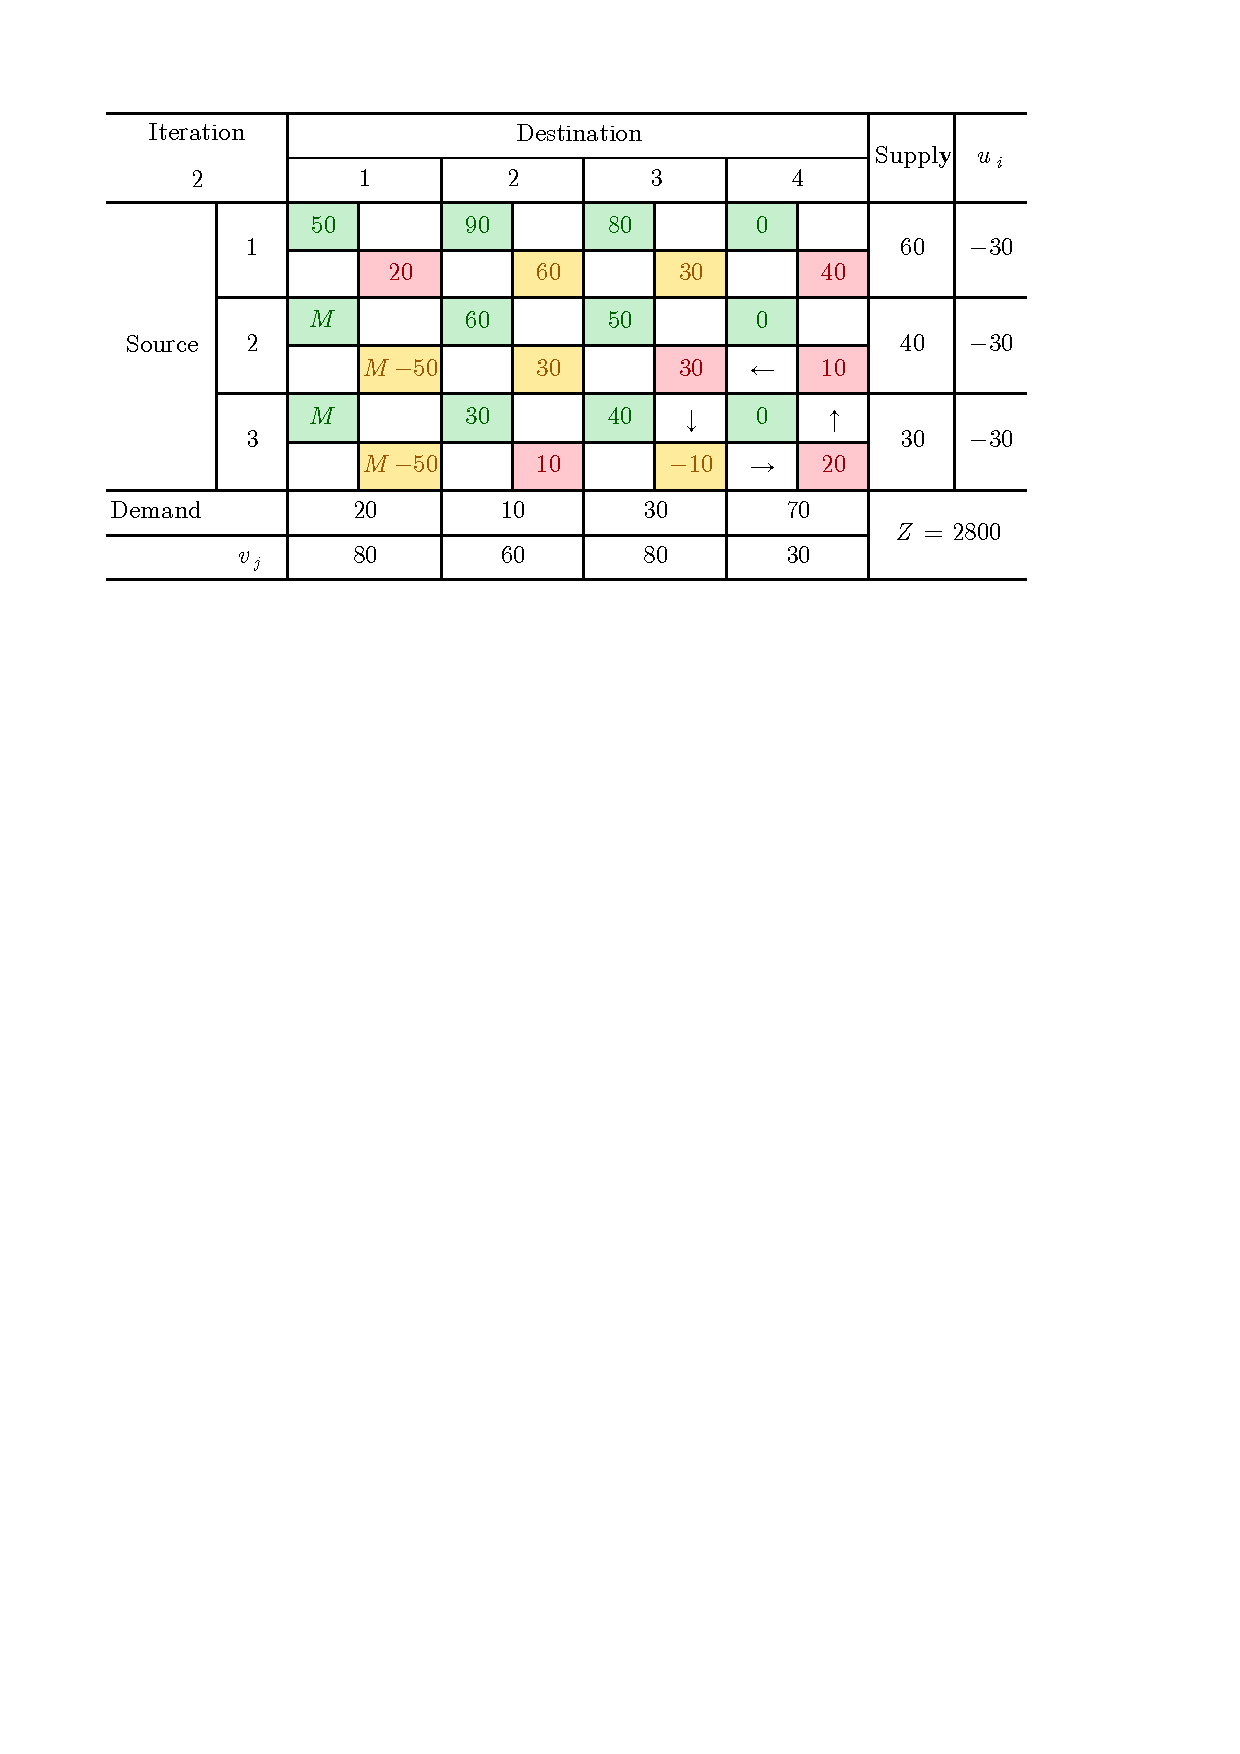
\includegraphics[width = 0.75\textwidth]{NW4}				
		\end{table}

	
		\begin{table}[H]
		\caption{Third iteration of transportation simplex tableau}
		\label{tabNW5}
		\centering
		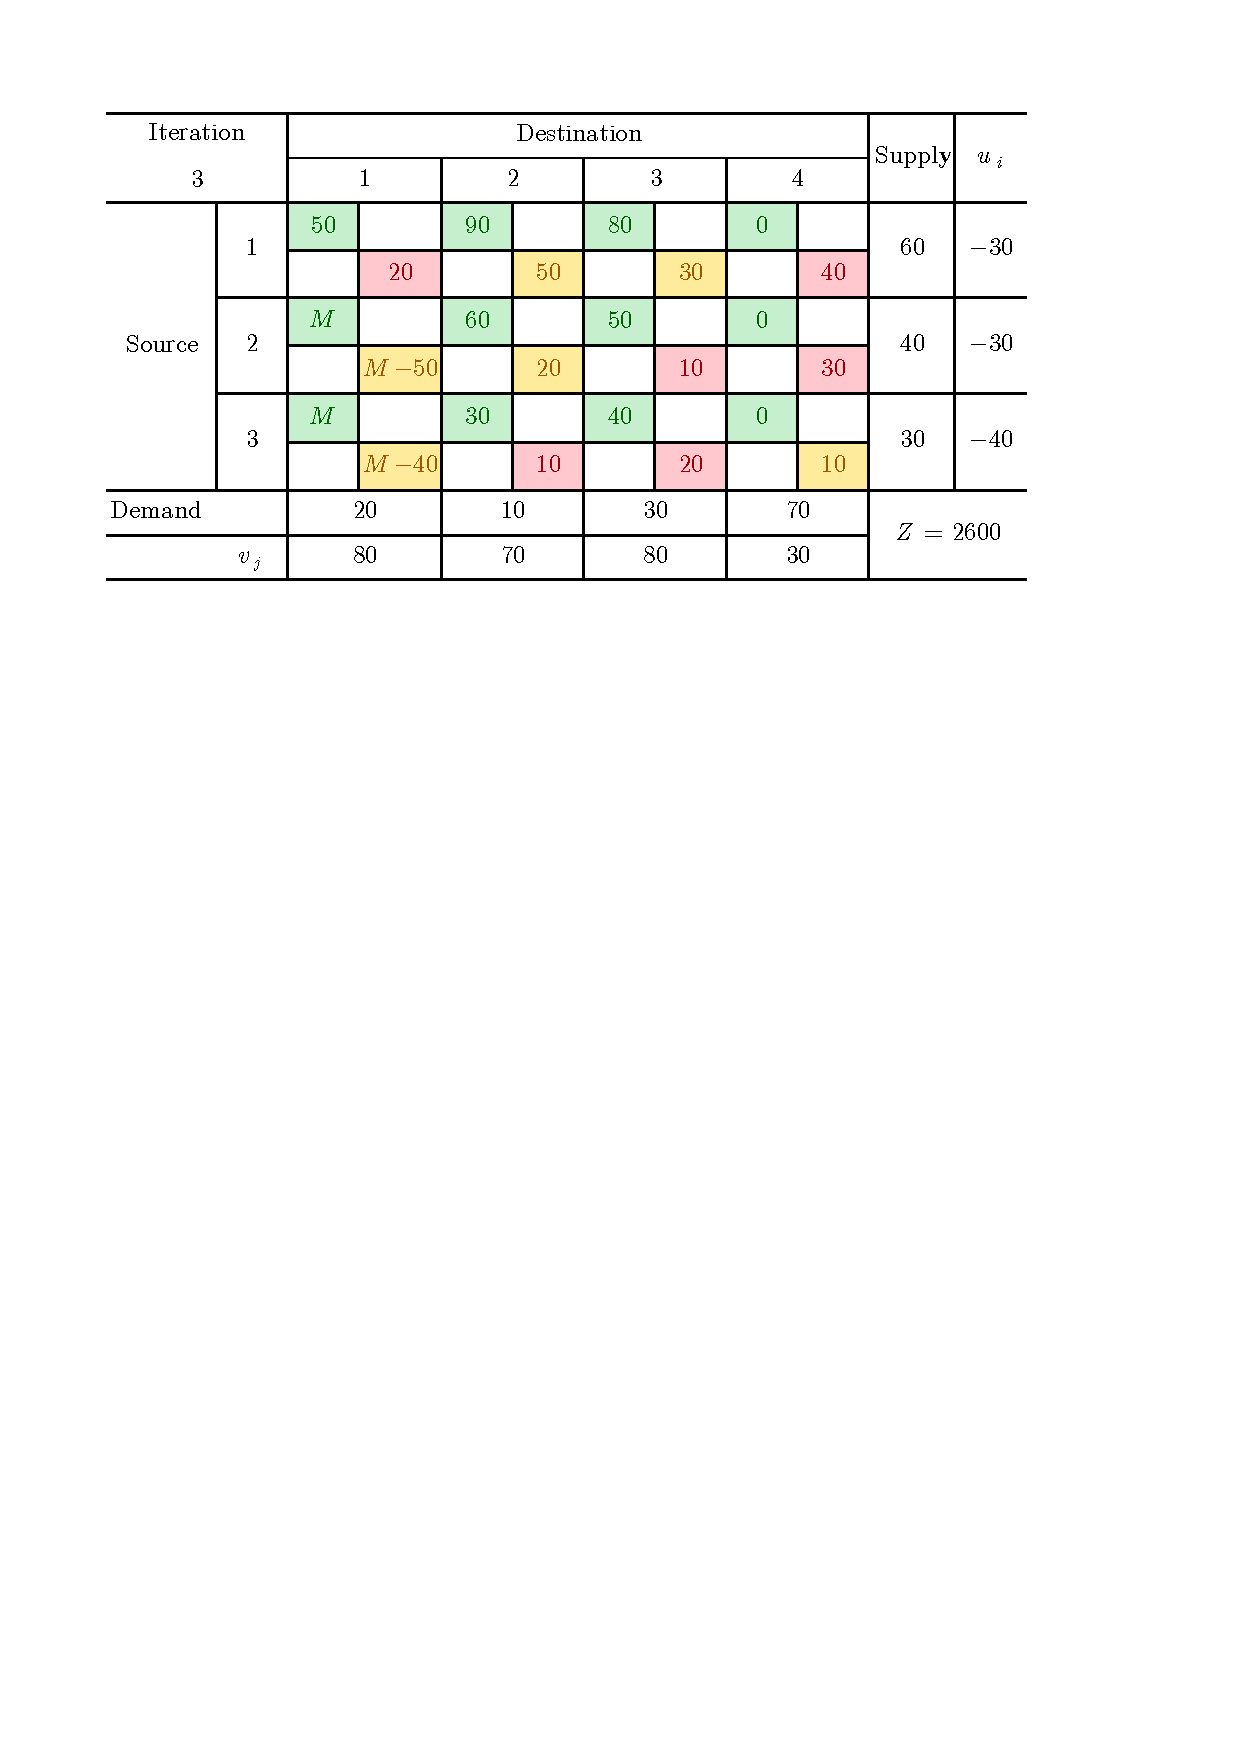
\includegraphics[width = 0.75\textwidth]{NW5}				
	\end{table}
\vspace*{-0.5cm}
		
		The optimal solution is 
		\begin{equation*}
		\begin{aligned}
		x_{11}&=20,\ x_{14}=40,\ x_{23}=10,\ x_{24}=30,\ x_{32}=10,\ x_{33}=20,\\
		x_{ij}&=0,\ \text{otherwise},
		\end{aligned}
		\end{equation*}
		with $Z=2600$.
		
	\end{solution}
	
	\item Use Vogel's approximation method to obtain an initial BF solution for this problem, and identify whether the initial BF solution is optimal. If the initial BF solution is not optimal, start with it and complete the first iteration of the transportation simplex method.
	\begin{solution}
		
		The initial BF solution obtained by Vogel's approximation method is shown from Tab.\ref{tabVO1} to Tab.\ref{tabVO5}. The selected row difference or column difference is in pink, while the selected cell is in green.
		\begin{table}[H]
			\caption{First step of Vogel's approximation method}
			\label{tabVO1}
			\centering
			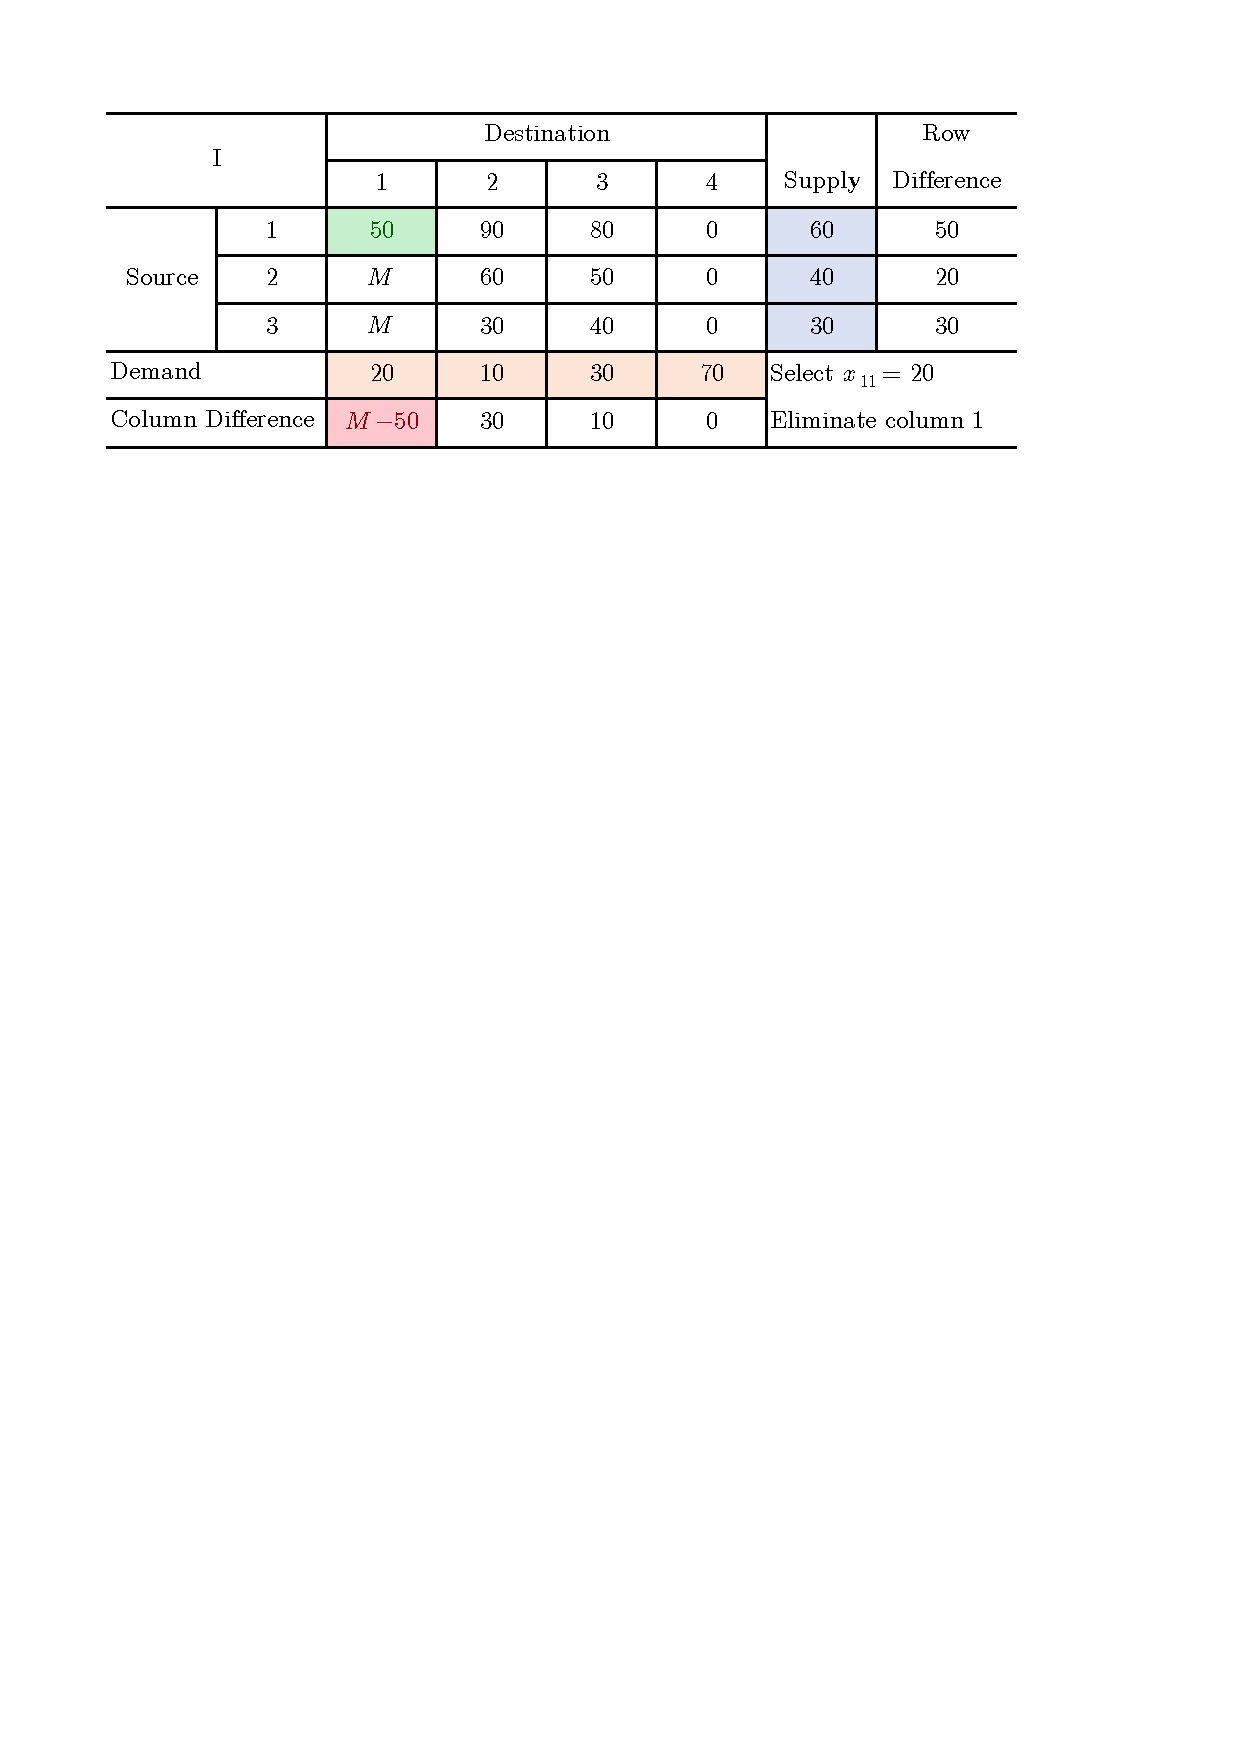
\includegraphics[width = 0.8\textwidth]{VO1}				
		\end{table}
	
	\begin{table}[H]
		\caption{Second step of Vogel's approximation method}
		\label{tabVO2}
		\centering
		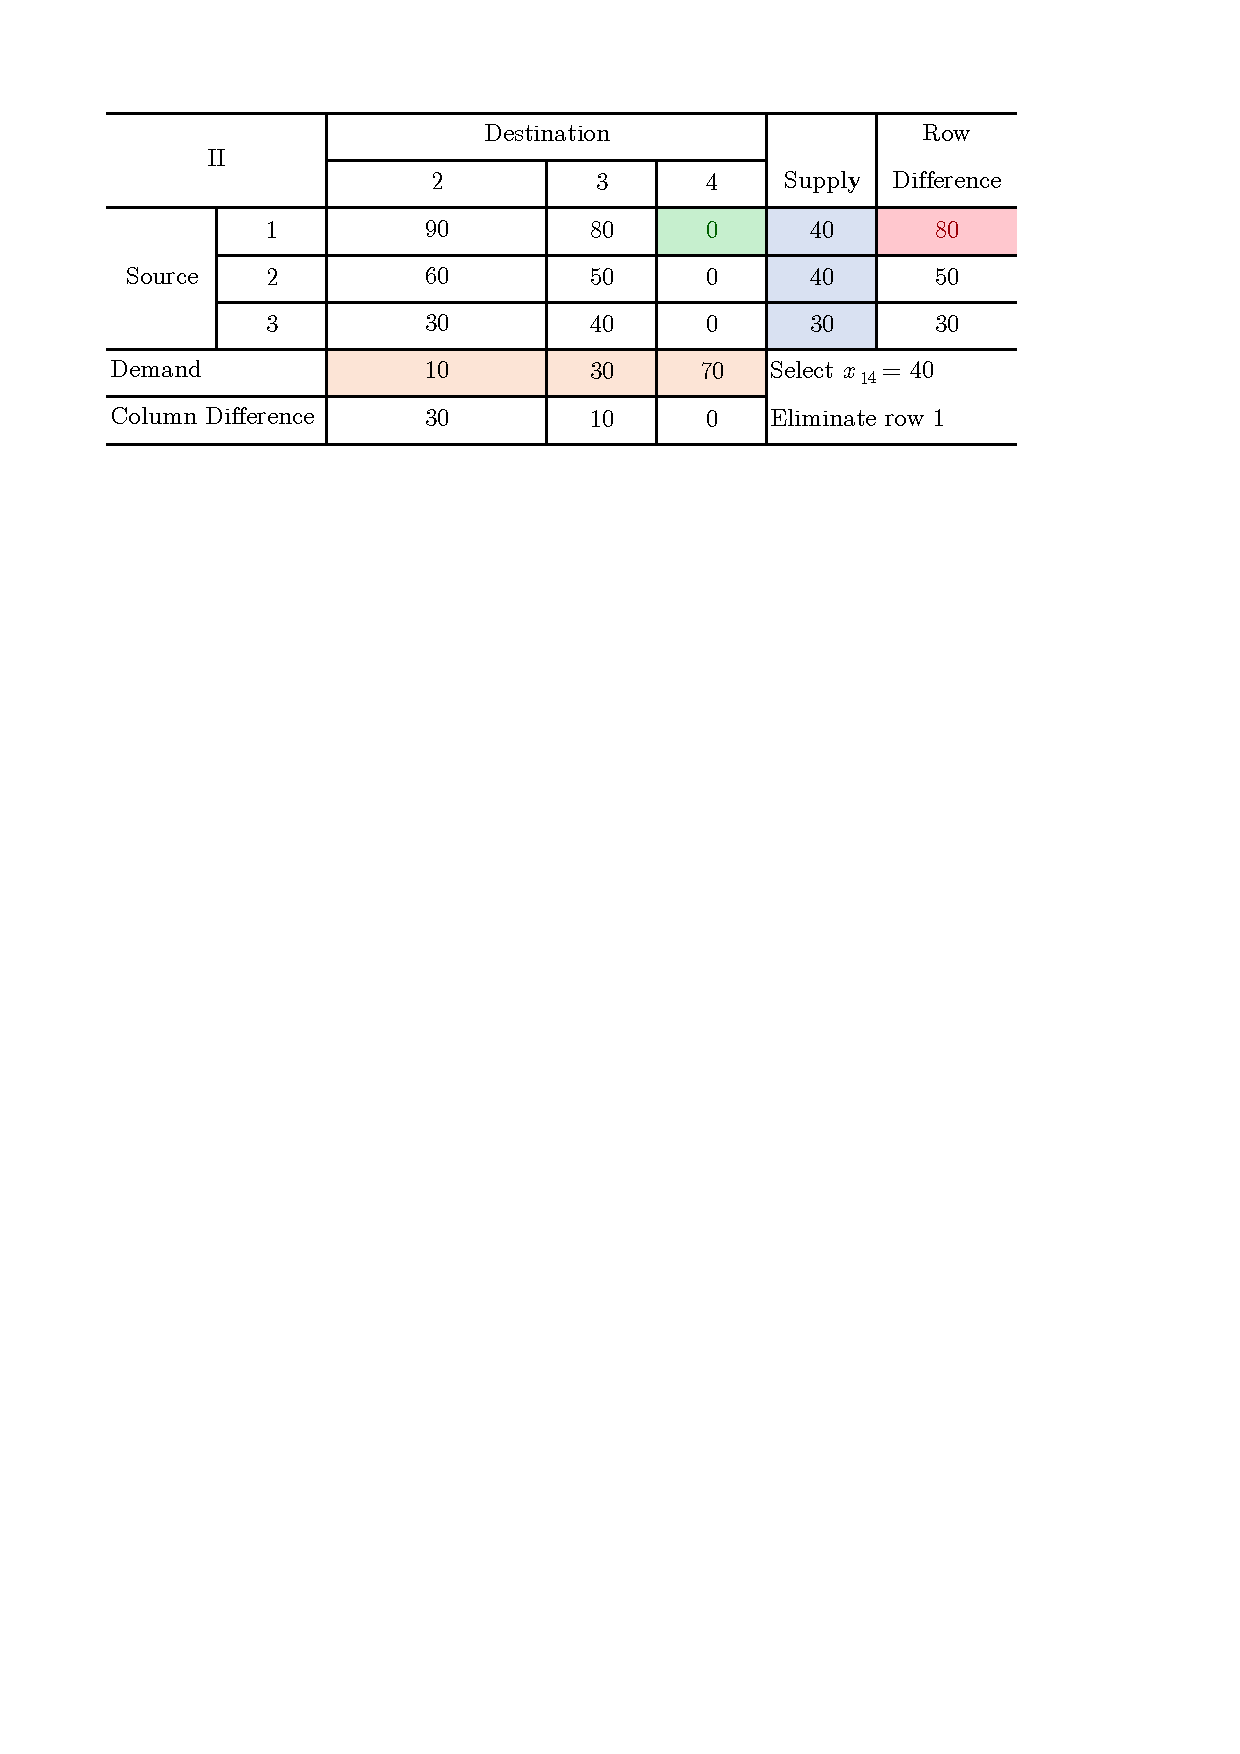
\includegraphics[width = 0.8\textwidth]{VO2}				
	\end{table}

	\begin{table}[H]
		\caption{Third step of Vogel's approximation method}
		\label{tabVO3}
		\centering
		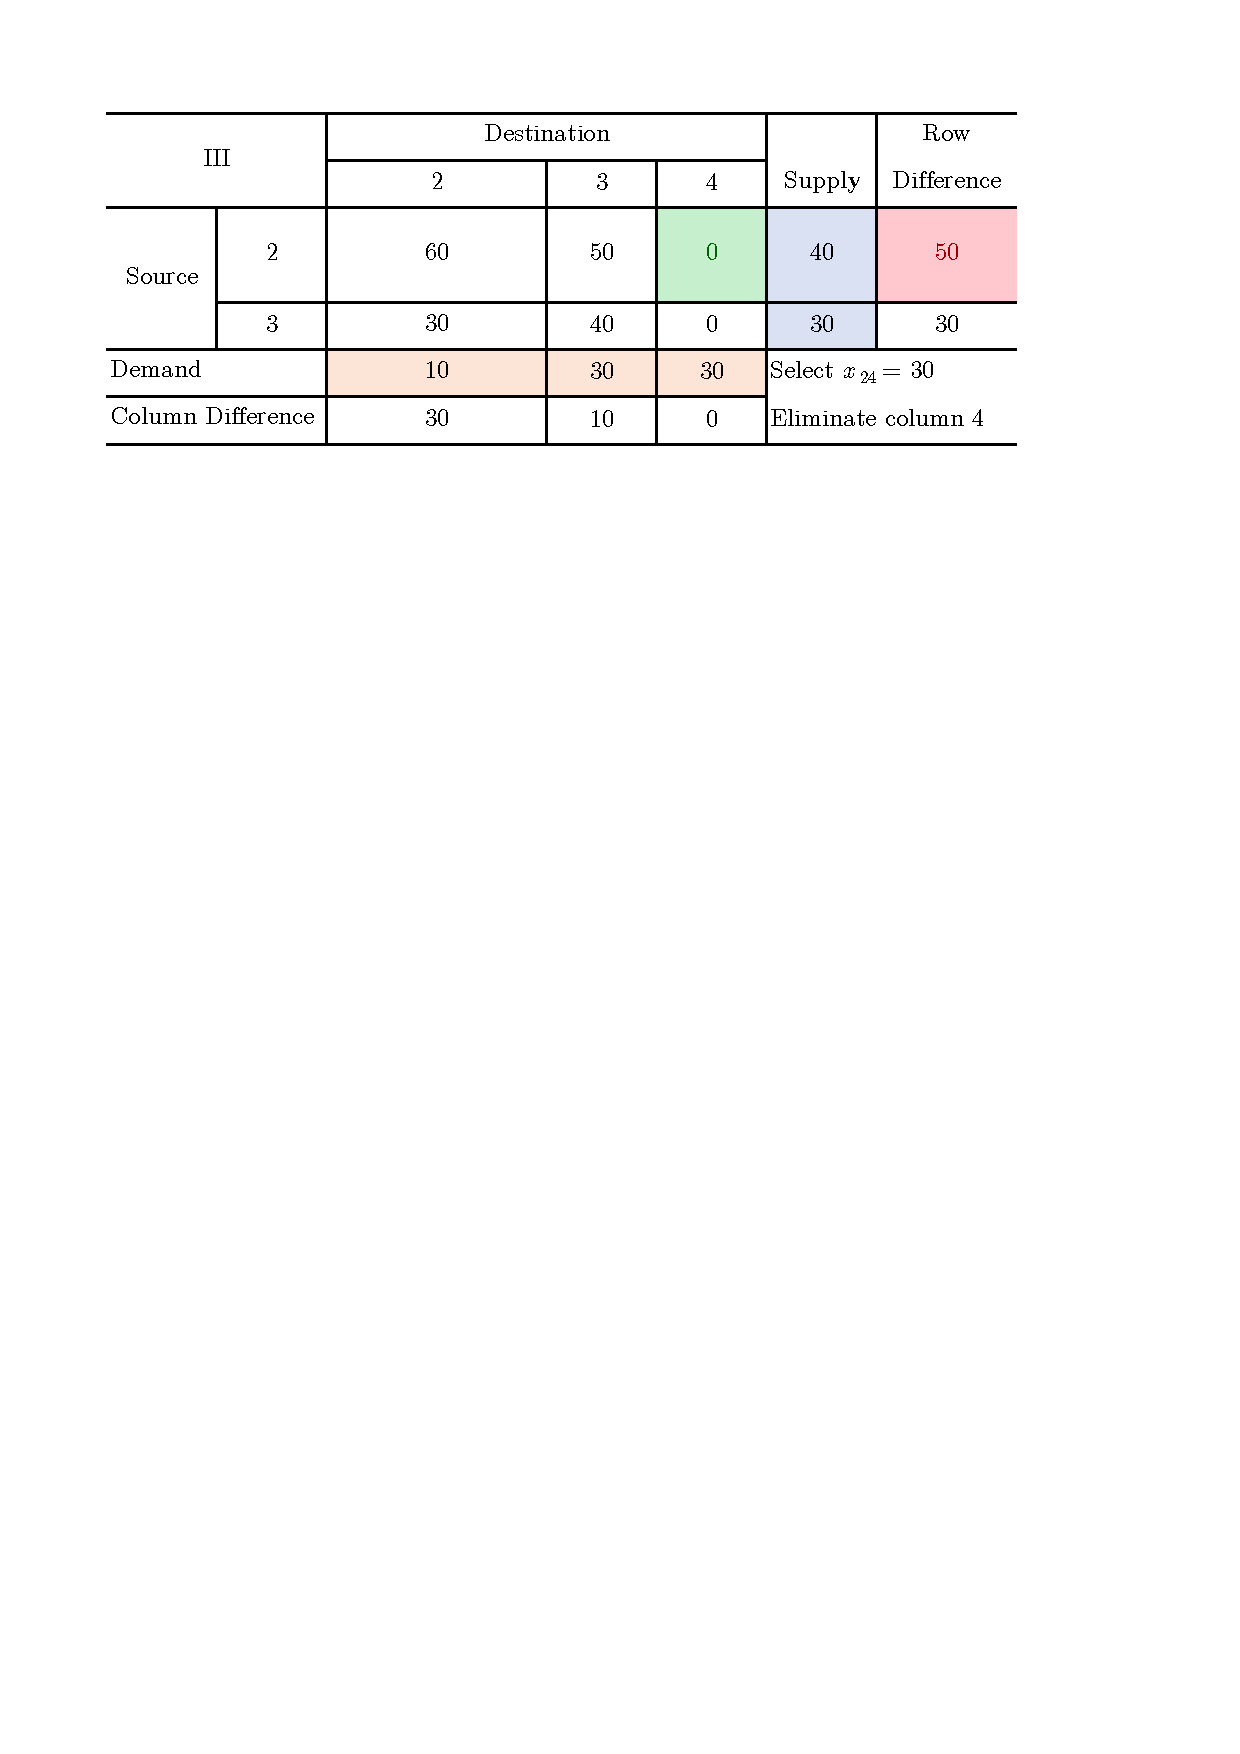
\includegraphics[width = 0.8\textwidth]{VO3}				
	\end{table}

	\begin{table}[H]
		\caption{Fourth step of Vogel's approximation method}
		\label{tabVO4}
		\centering
		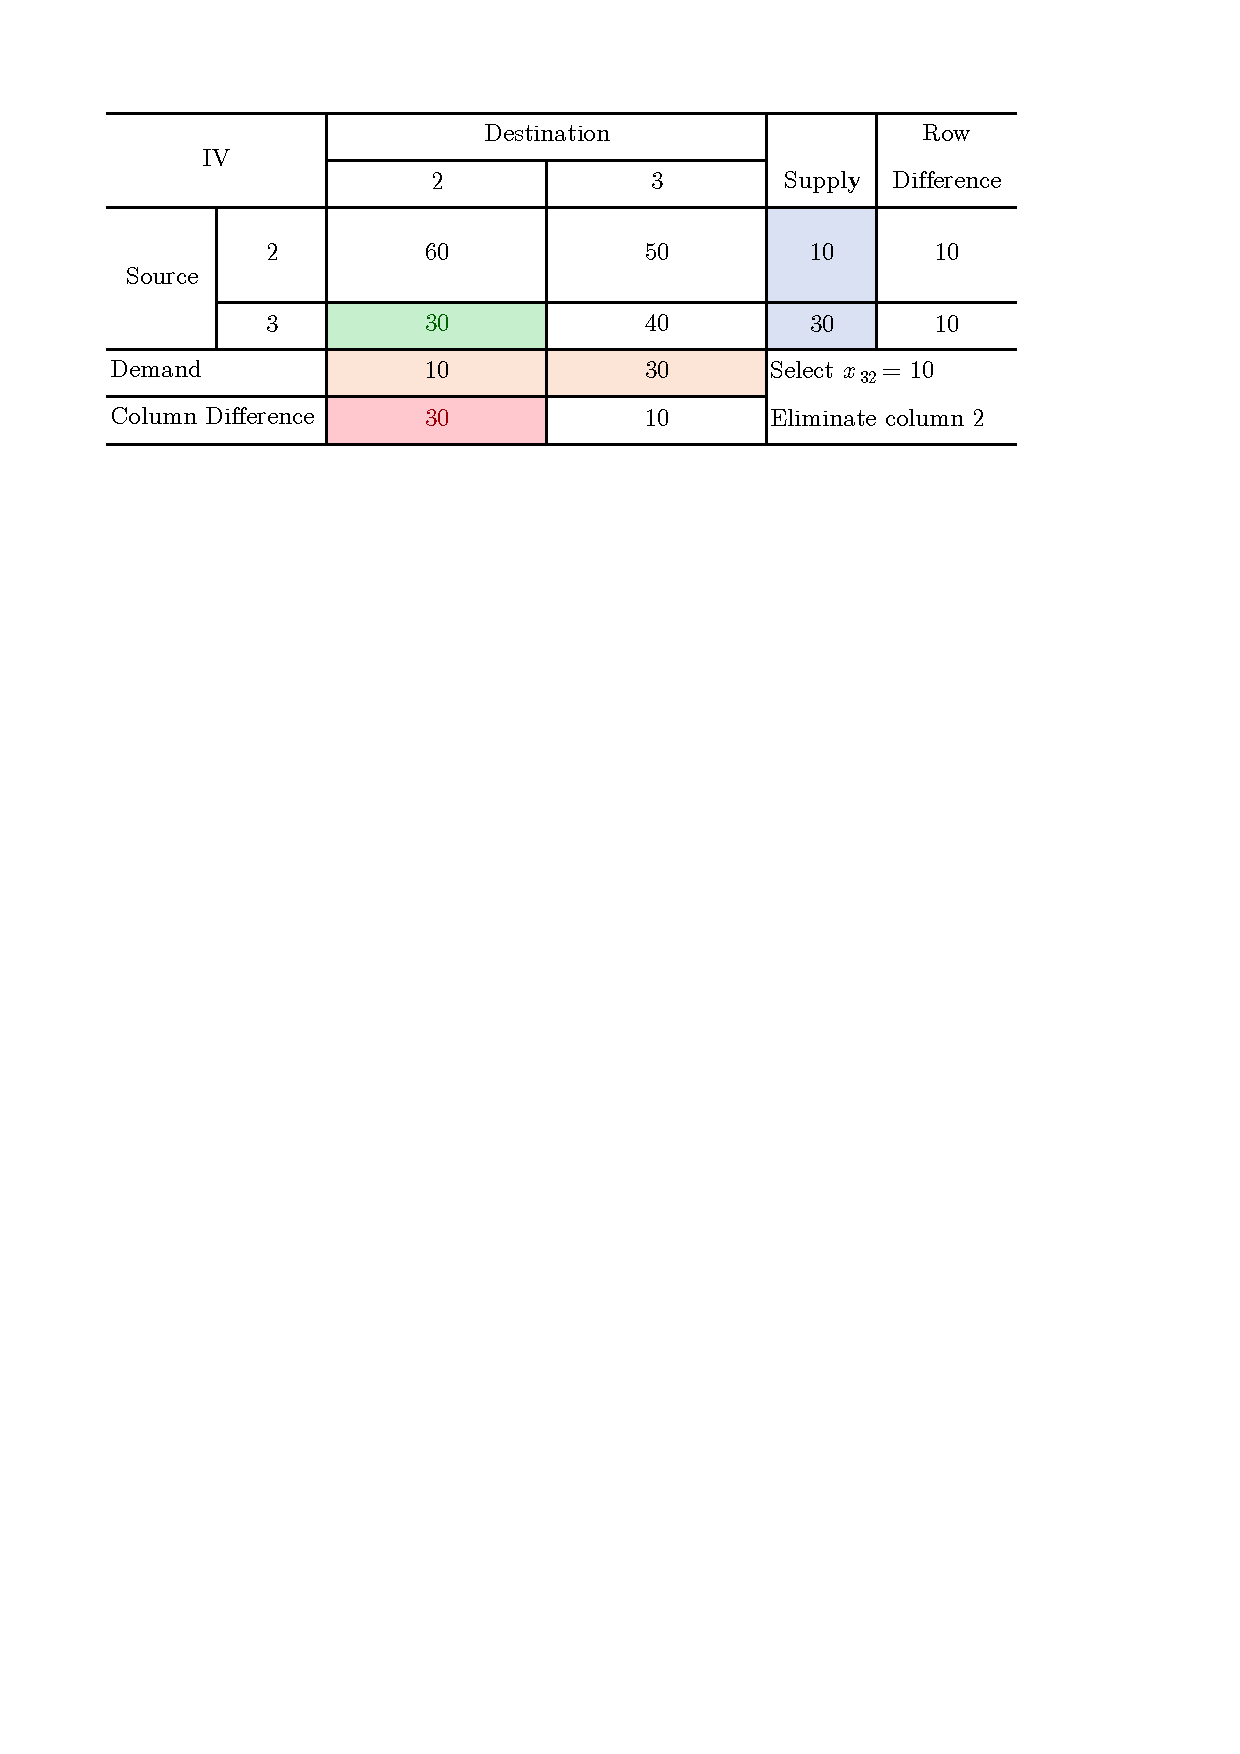
\includegraphics[width = 0.8\textwidth]{VO4}				
	\end{table}

	\begin{table}[H]
		\caption{Fifth step of Vogel's approximation method}
		\label{tabVO5}
		\centering
		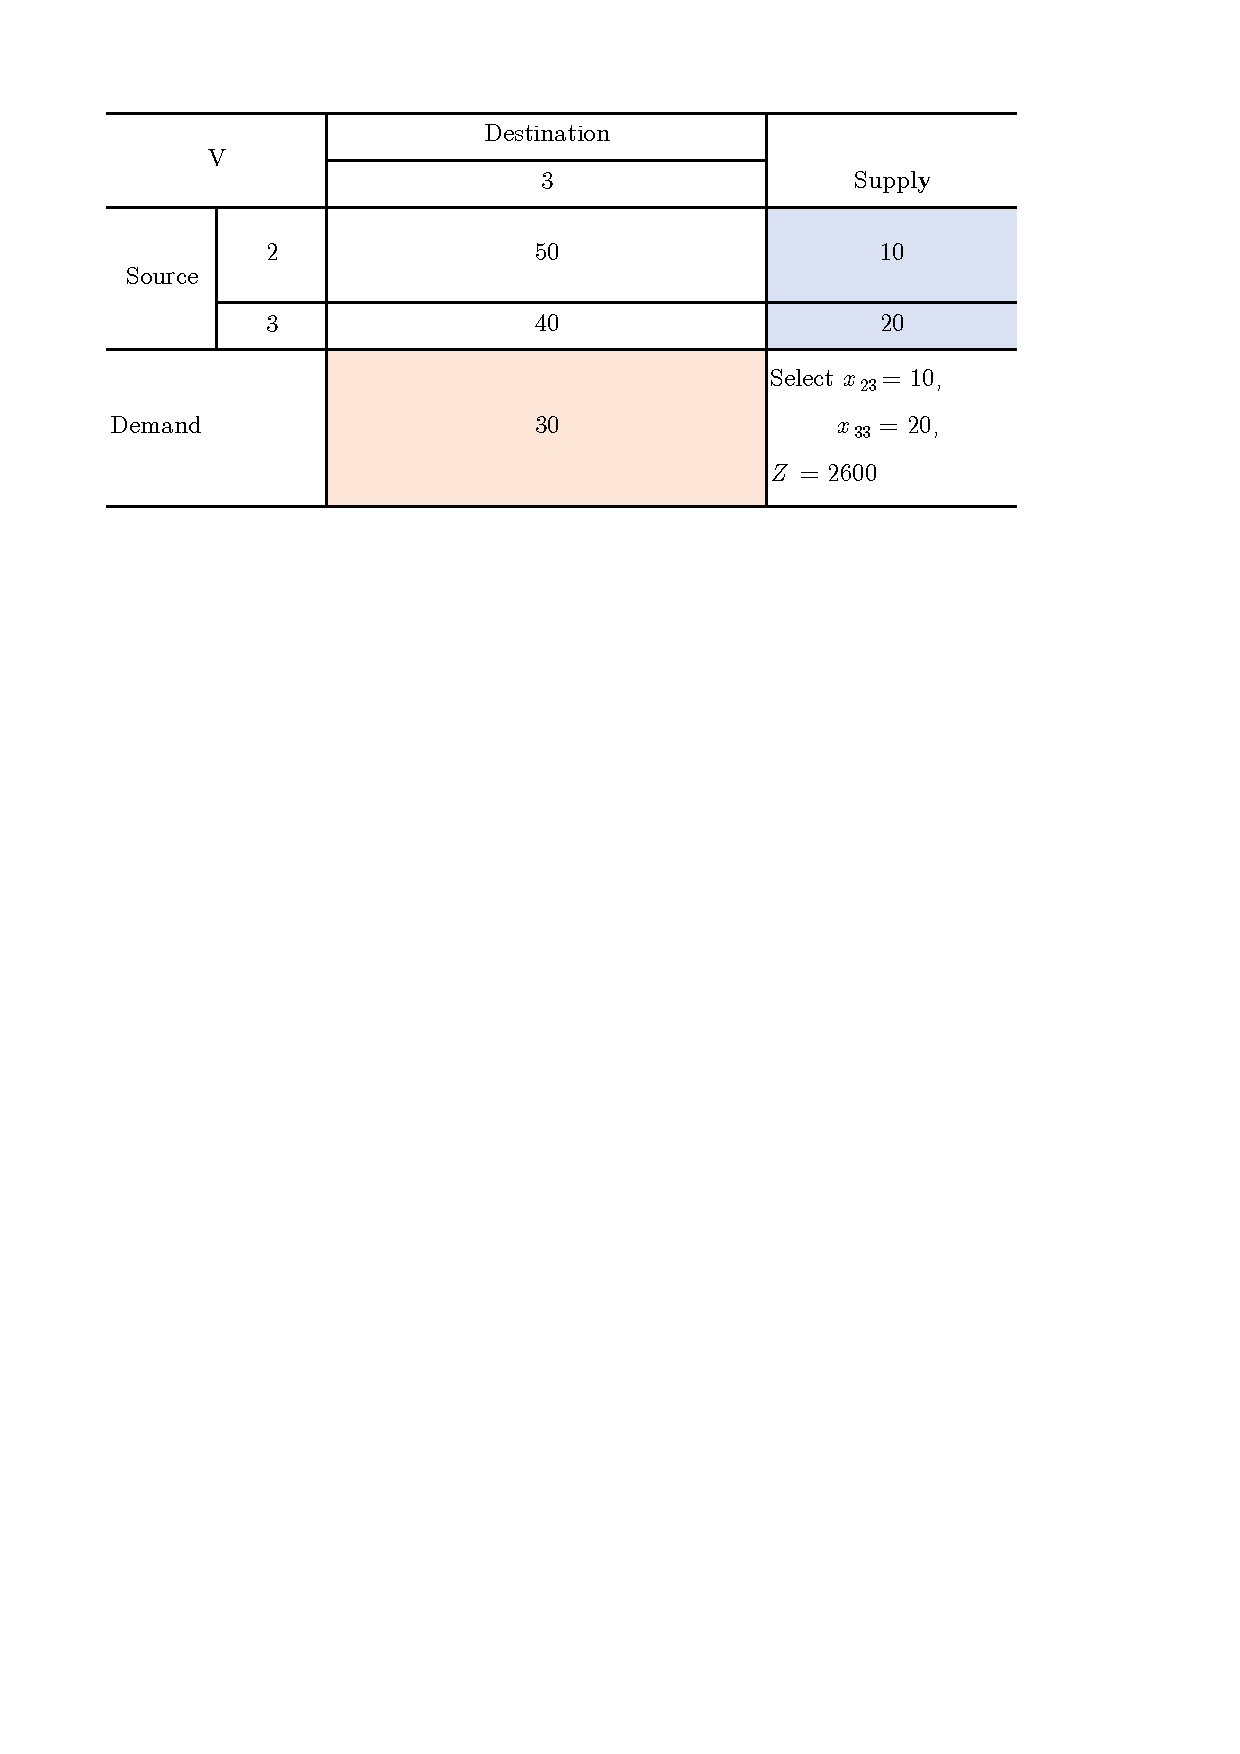
\includegraphics[width = 0.8\textwidth]{VO5}				
	\end{table}
	
	Therefore, the initial BF solution is 
	\begin{equation*}
	\begin{aligned}
	x_{11}&=20,\ x_{14}=40,\ x_{23}=10,\ x_{24}=30,\ x_{32}=10,\ x_{33}=20,\\
	x_{ij}&=0,\ \text{otherwise},
	\end{aligned}
	\end{equation*}
	with $Z=2600$, which is the optimal solution just found in Tab.\ref{tabNW5} of question (b).
	
	\newpage
	\textit{Optimality test}
	
	The optimality test result is shown in Tab.\ref{tabVOOP}. Since all nonbasic variables are positive, the initial BF solution is the optimal solution.
	
	\hspace*{4ex}What's more, comparing Tab.\ref{tabNW5} and Tab.\ref{tabVOOP}, we can see that the assignment of the first value for $u_i$ or $v_j$ will not change the value of nonbasic variables.
	
	\begin{table}[H]
		\caption{Optimality test of the initial BF solution}
		\label{tabVOOP}
		\centering
		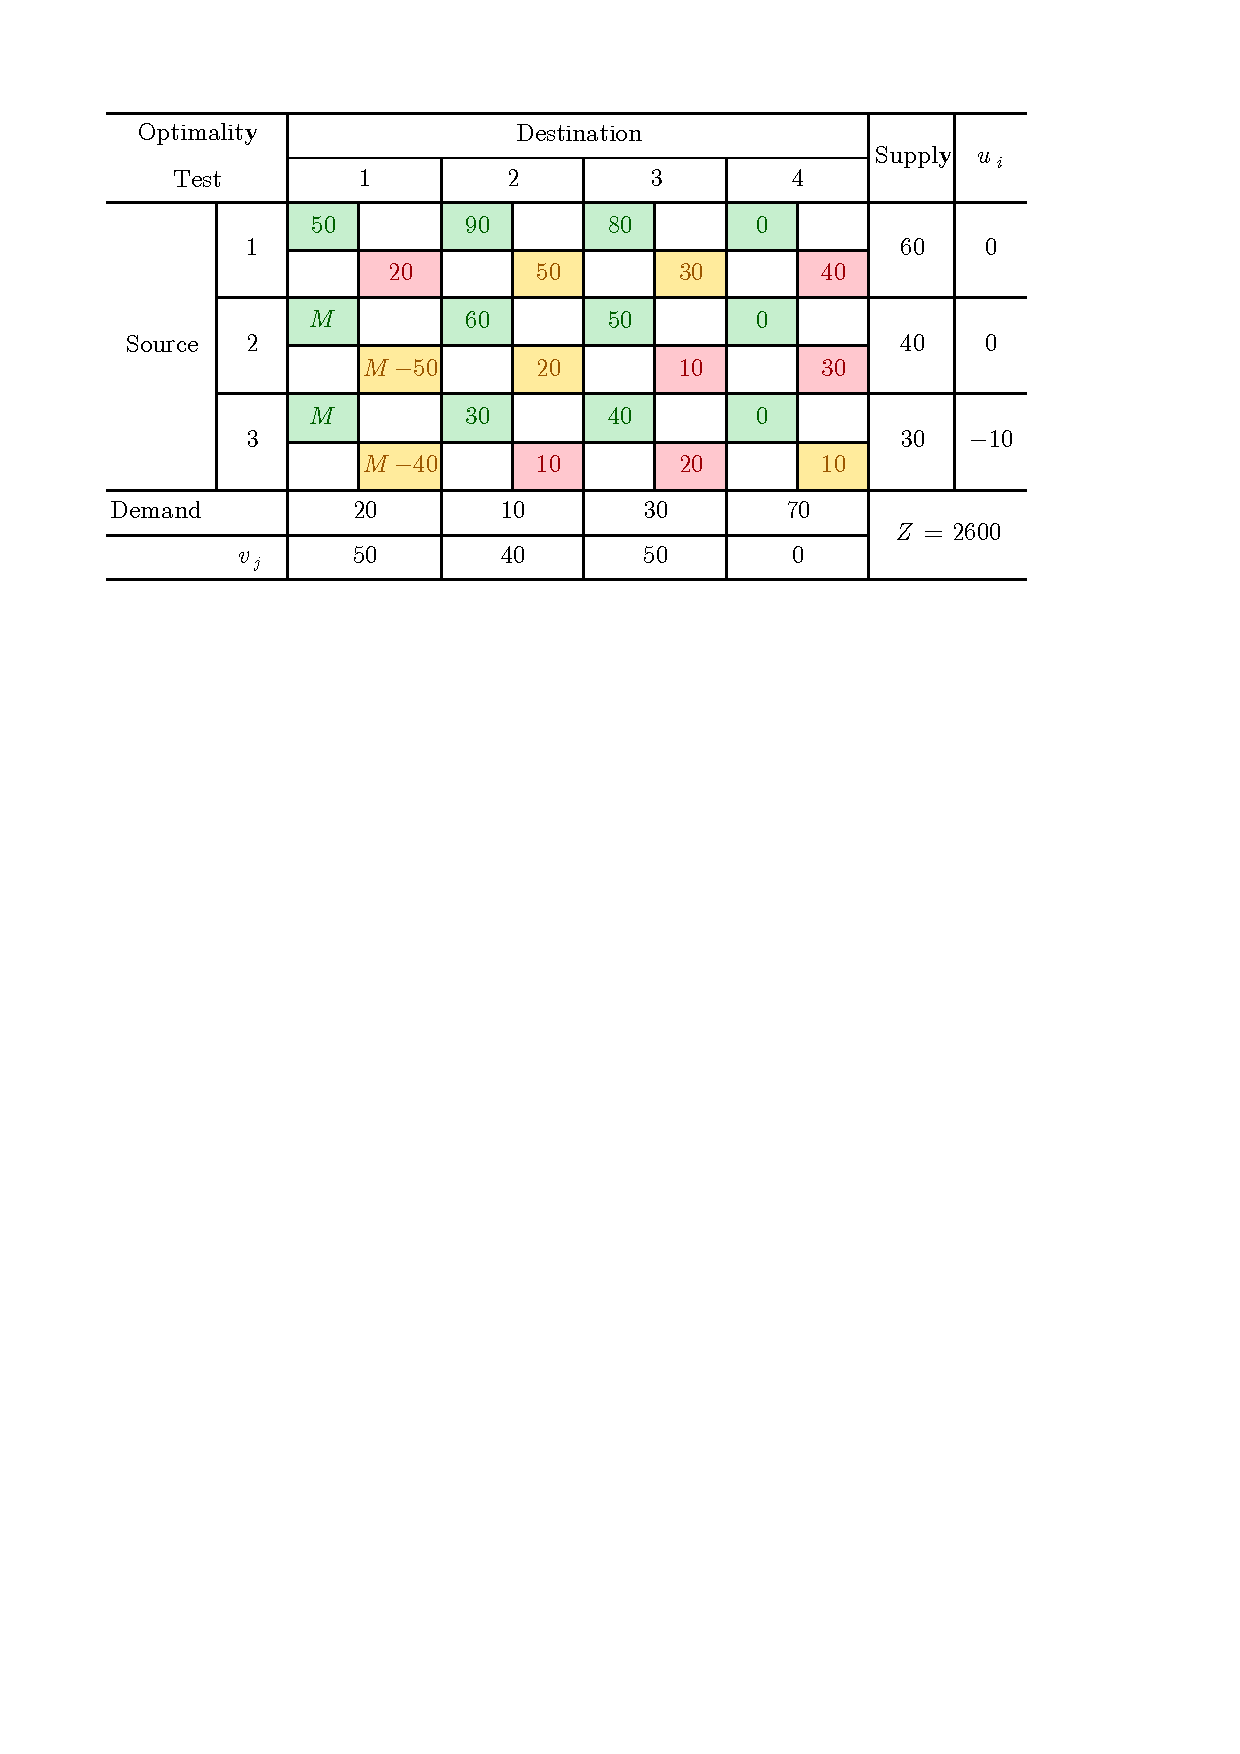
\includegraphics[width = 0.8\textwidth]{VOOP}				
	\end{table}
	
	\end{solution}
\end{enumerate}


% w.r.t the external
\end{enumerate}
%  The source code to plot Figure \ref{fig:1} could be found in Appendix \ref{sec:a:code}. Here are the core codes:
%  \lstinputlisting[firstline=6,lastline=7, firstnumber=6]{matlabscript.m}

%  \newpage
%  \appendix
%  \section{Source code}
%  \label{sec:a:code}
%  % \lstlistoflistings
%  Source code for plotting Figure \ref{fig:1} is shown as follows.
%  \lstinputlisting[caption=FigurePlot]{matlabscript.m}
  
\end{document}
